\documentclass{jarticle}

\usepackage{twocolumn}
% \usepackage[dvi ps]{graphicx}%%画像を読み込む
\usepackage[dvipdfmx]{graphicx}
\usepackage{subfigure}
\usepackage{amsmath}          %%genfrac http://www.biwako.shiga-u.ac.jp/sensei/kumazawa/tex/form006.html
\usepackage{ulem}             %%http://biwako.shiga-u.ac.jp/sensei/kumazawa/tex/ulem.html     uline,uuline,uwave,sout,xoutなど
\usepackage{multirow}
\usepackage{here}
% \usepackage{setspace}
\usepackage{chukan2018}       %%最後に読み込むこと!(最後に読み込まないと\textwidthなどの設定が反映されない)

\pagestyle{empty} %ページ番号を入れるときにはコメントアウトする

\begin{document}

\linesparpage{50}

\title{
筋配置を最適化したカニ模倣ロボットの開発
}
\etitle{
Development of a crab-mimicking robot with optimized muscle placement
}
\author{
研究者 濱口 紘生  指導教員  中西 大輔
}
\eauthor{
Keywords: McKibben Pneumatic Actuater, Exoskeleton, Biomimetic Robot
}

\maketitle

\thispagestyle{empty}  %1ページ目にページ番号を入れるときにはコメントアウトする

%%%%%%%%%%%%%%%%%%%%%%%%%%%%%%%%%%%%%%%%%%%%%%%%%%%%%%%%%%%%%%%%%%%%%%%%%%%%%%%
\section{緒言}

代表的な人工筋肉として,圧縮空気を印加することにより骨格筋のように収縮するMcKibben型人工筋肉(MPA)
があげられる.従来は直径が数十mm程度のものが多かったが,近年では数mm程度のMPAが注目を集めている\cite{wakimoto}.
その細さを生かして小さい筋肉,あるいは集積によって単純な紡錘形以外の筋肉を表現可能なことから,筋骨格系ロボットにおいて特盛んに用いられている\cite{wakimoto}.
一方で,甲殻類をはじめとする外骨格を有する生物模倣ロボットについては,ワイヤ駆動や関節にサーボモータを配置したものが主流であった\cite{crabrobot1}.
これは外骨格内部にアクチュエータを配置するのが困難なためである.細径MPAであれば骨格内部にアクチュエータを配置することが可能であり,
実際の生物に近い構成でロボットを作成することが可能である.そこで本研究では外骨格生物のうち甲殻類の蟹をモデルに,
実際の蟹の筋肉と関節の構造を参考にして細径MPAを使用した蟹の歩脚ロボットの開発に取り組む.

%%%%%%%%%%%%%%%%%%%%%%%%%%%%%%%%%%%%%%%%%%%%%%%%%%%%%%%%%%%%%%%%%%%%%%%%%%%%%%%
\vspace*{-2mm}
\section{MPAおよび蟹模倣ロボットについて}

\vspace*{-1mm}
\subsection{細径MPAについて}

従来のMPAと細径MPAを図\ref{fig:MPA}に示す.細径MPAの特徴として以下の点が挙げられる.1つ目に細くて軽量のため限られた狭いスペースへの配置と集積が可能,2つ目に集積化により収縮量を増大させること,
3つ目に集積化により羽状筋のような複雑な筋肉の再現が可能であることである.

%%%%%%%%%%%%%%%%%%%%%%%%%%%%%%%%%%%%%%%%%%%%%%%%%%%%%%%%%%%%%%%%%%%%%%%%%%%%%%%
\vspace*{-1mm}
\subsection{細径MPAを用いた蟹模倣ロボットについて}

細径MPAを用いて作成された蟹模倣ロボットを図\ref{fig:crabrobot}に示す.ここでは,細径MPAを腱に対して斜めになるように集積して蟹の羽状筋を再現している.
これにより,0.4MPaの圧縮空気を印加すると開閉動作を確認することができた.しかし,本来の蟹の関節の可動域を完全には再現できていなかった.
考えられる原因は3つある.1つ目に細径MPAの端部が角度を自由に変化できない部品であったため,細径MPAが収縮して腱を引き込んで角度が変わる際に端部から反対方向に力が加わってしまうこと.
2つ目に細径MPAが圧縮空気を印加していないとき,ナイロンメッシュとシリコンゴムチューブの間に隙間がありその分ストロークが減り収縮率が低下してしまっていたこと.
3つ目に今回蟹の解剖をして蟹の筋配置が腱の上側と下側で違っていることが判明し,それが図\ref{fig:crabrobot}のロボットでは再現できていなかったこと.
以上の3つのことが原因で本来の蟹の関節の可動域を再
%%%%%%%%%%%%%%%%%%%%%%%%%%%%%%%%%%%%%%%%%%%%%%%%%%%%%%%%%%%%%%%%%%%%%%%%%%%%%%%
\begin{figure}[H]
  \begin{minipage}[b]{0.47\columnwidth}
    \centering
    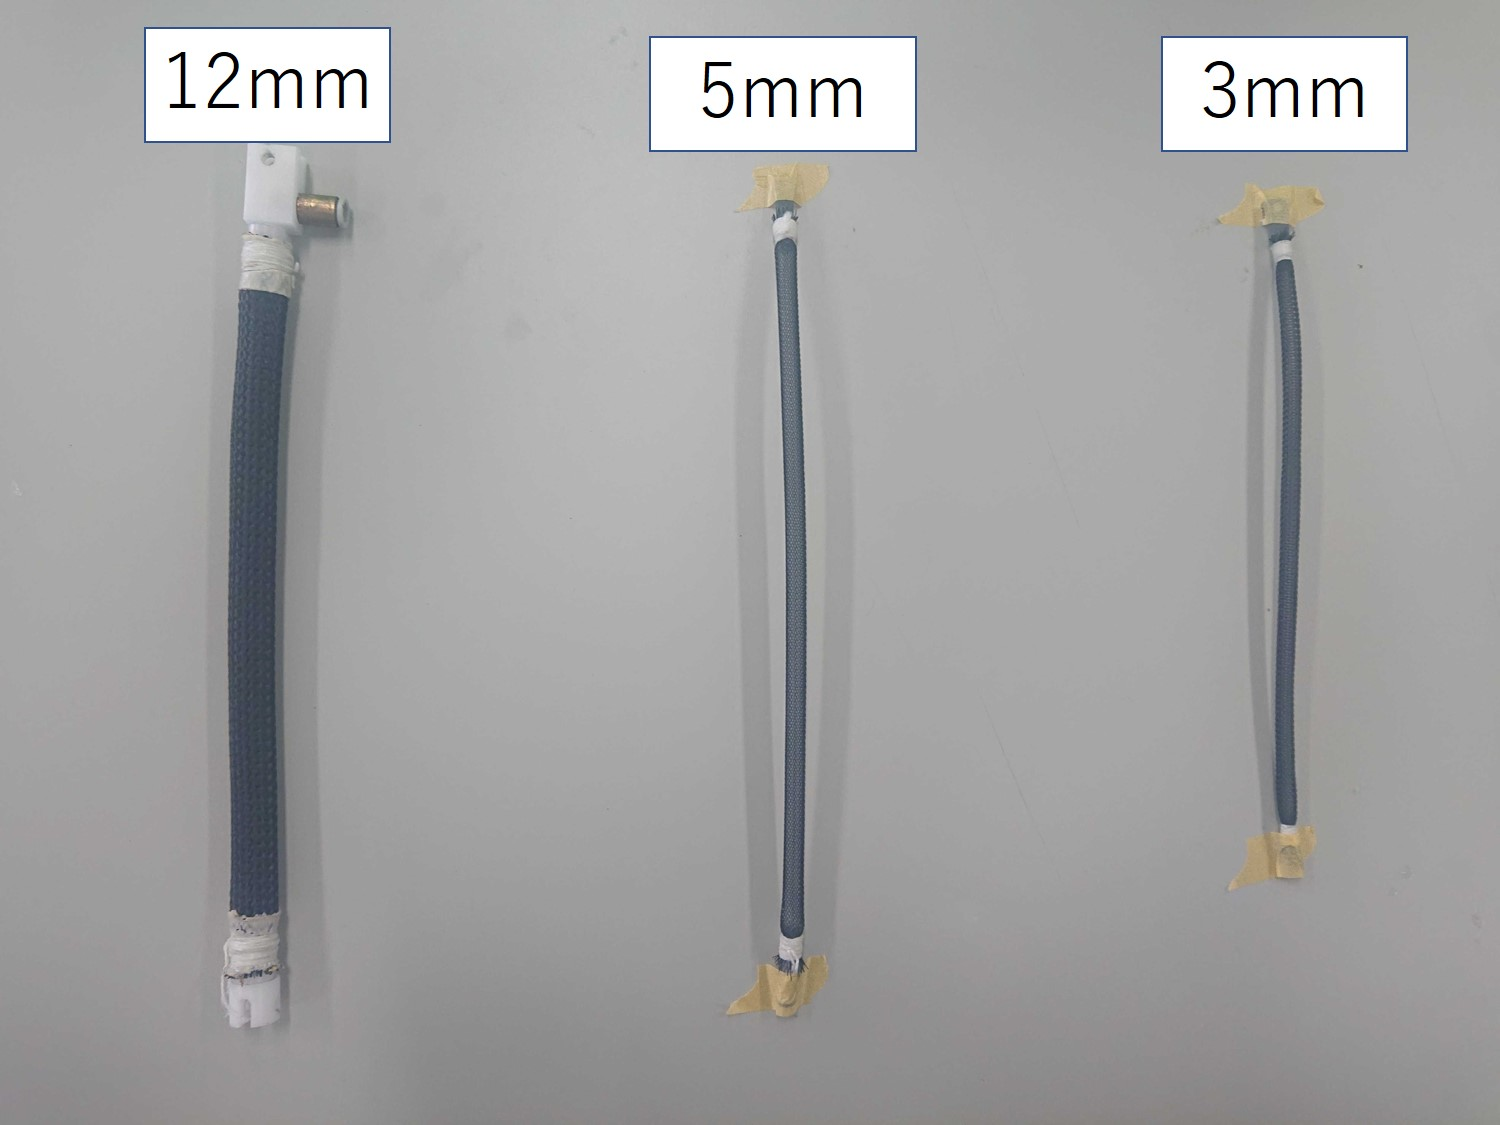
\includegraphics[scale=0.13]{mpa.JPG}
    \vspace{-4mm}
    \caption{MPAの外径}
    \label{fig:MPA}
  \end{minipage}
  \hspace{0.04\columnwidth}
  \begin{minipage}[b]{0.47\columnwidth}
    \centering
    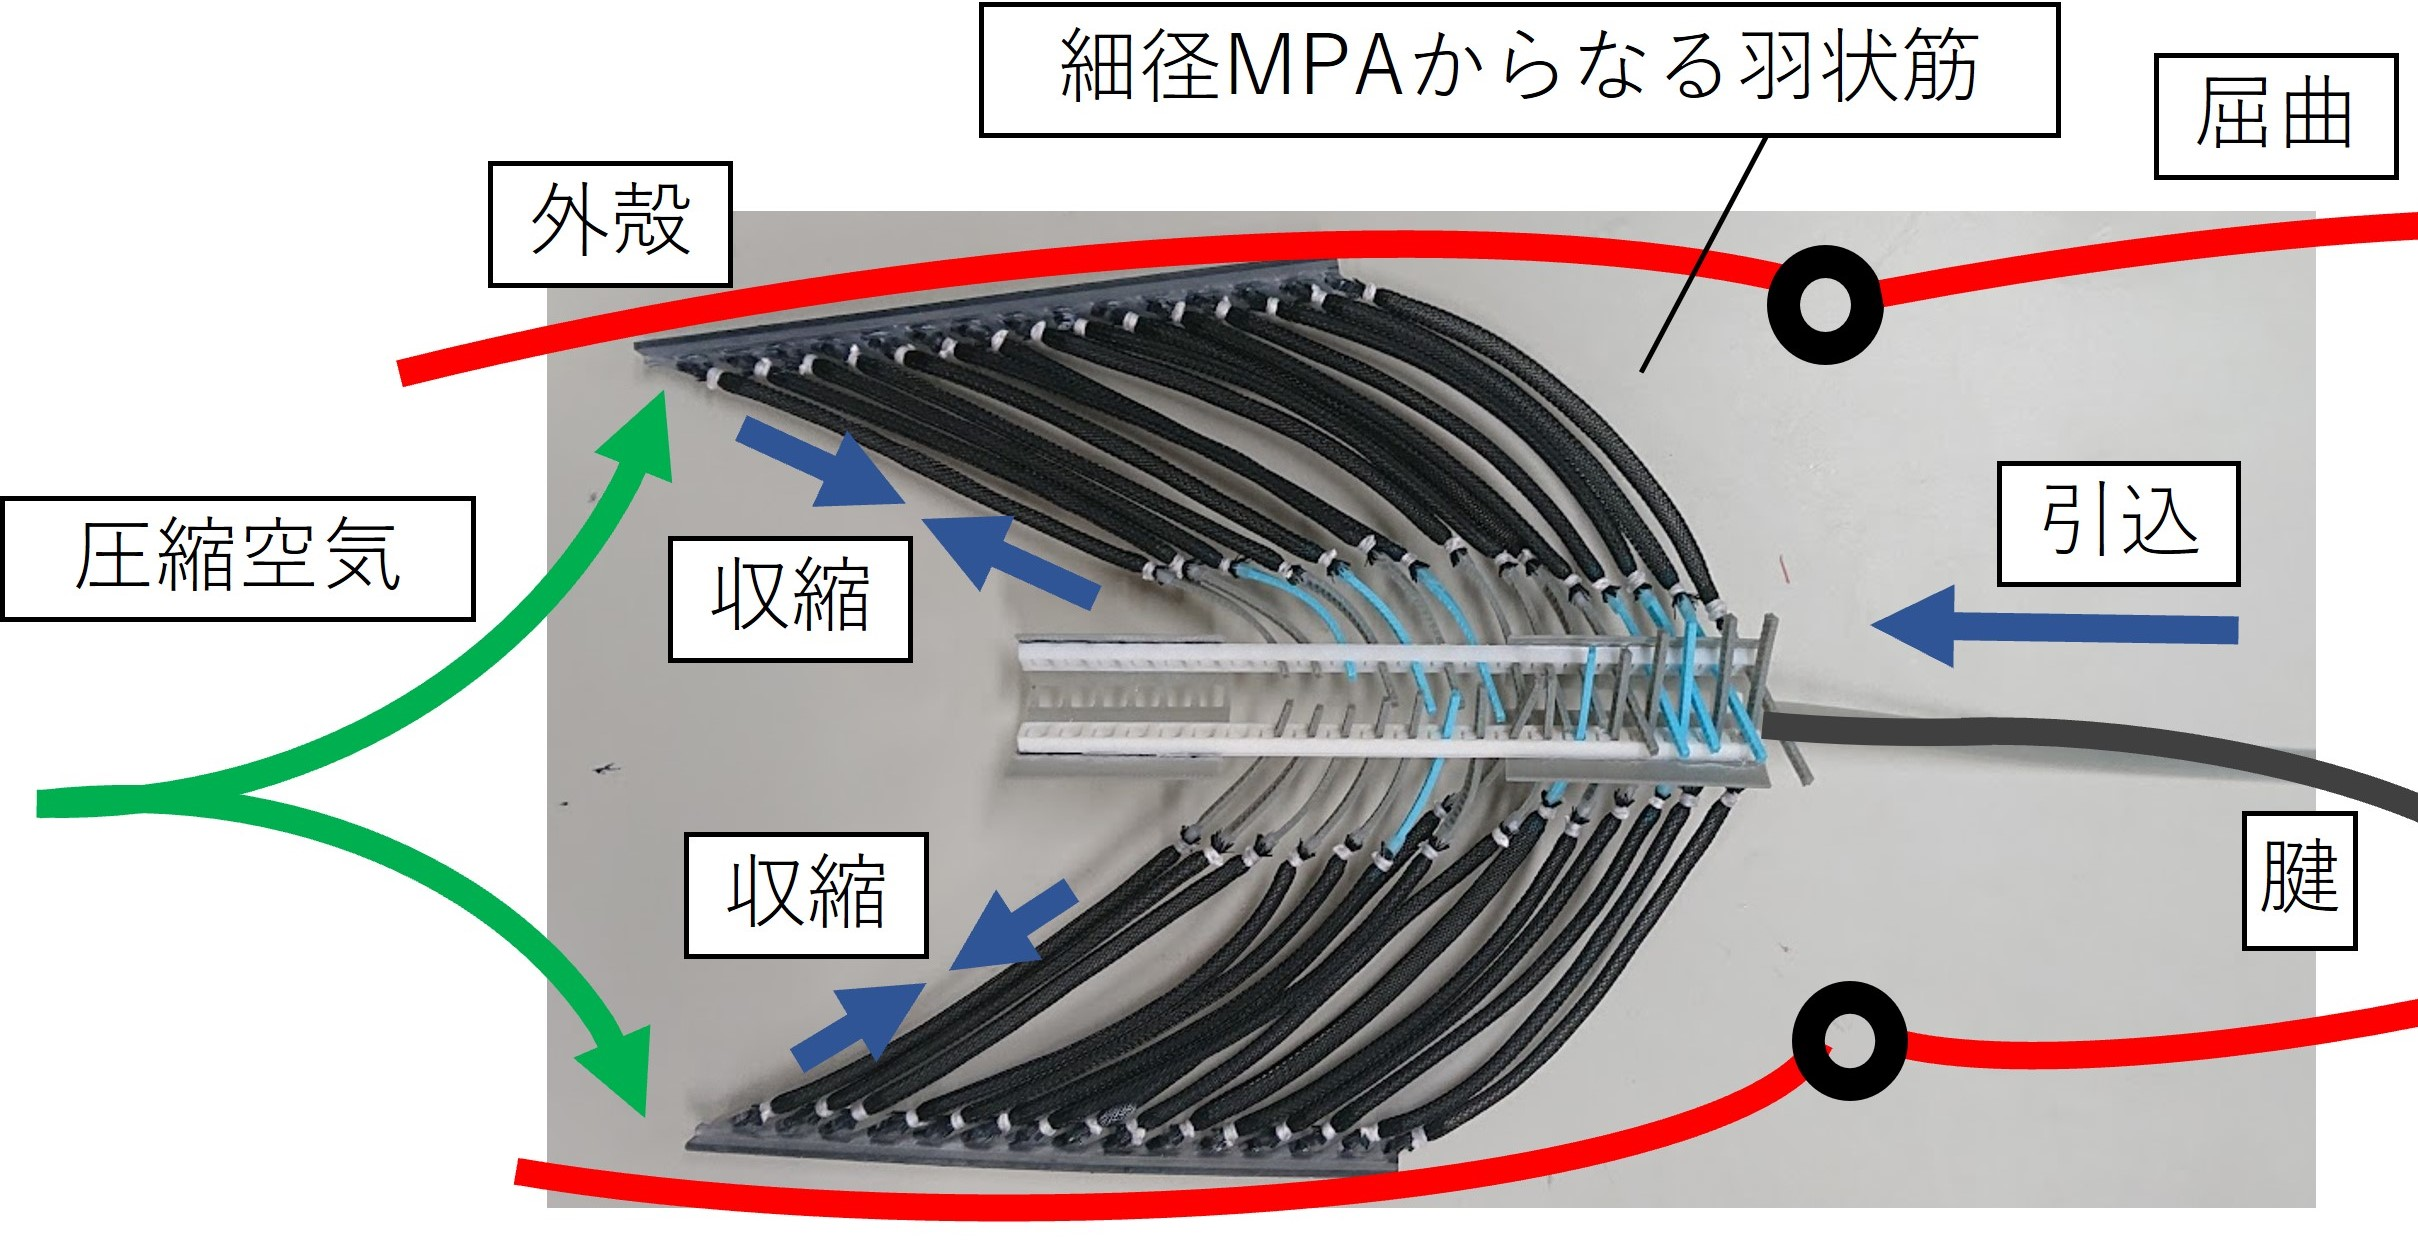
\includegraphics[scale=0.18]{mosiki.JPG}
    \vspace{-2mm}
    \caption{蟹模倣ロボット\cite{crabrobot2}}
    \label{fig:crabrobot}
  \end{minipage}
\end{figure}
%%%%%%%%%%%%%%%%%%%%%%%%%%%%%%%%%%%%%%%%%%%%%%%%%%%%%%%%%%%%%%%%%%%%%%%%%%%%%%%

%%%%%%%%%%%%%%%%%%%%%%%%%%%%%%%%%%%%%%%%%%%%%%%%%%%%%%%%%%%%%%%%%%%%%%%%%%%%%%%
\begin{figure}[H]
  \begin{minipage}[b]{0.47\columnwidth}
    \centering
    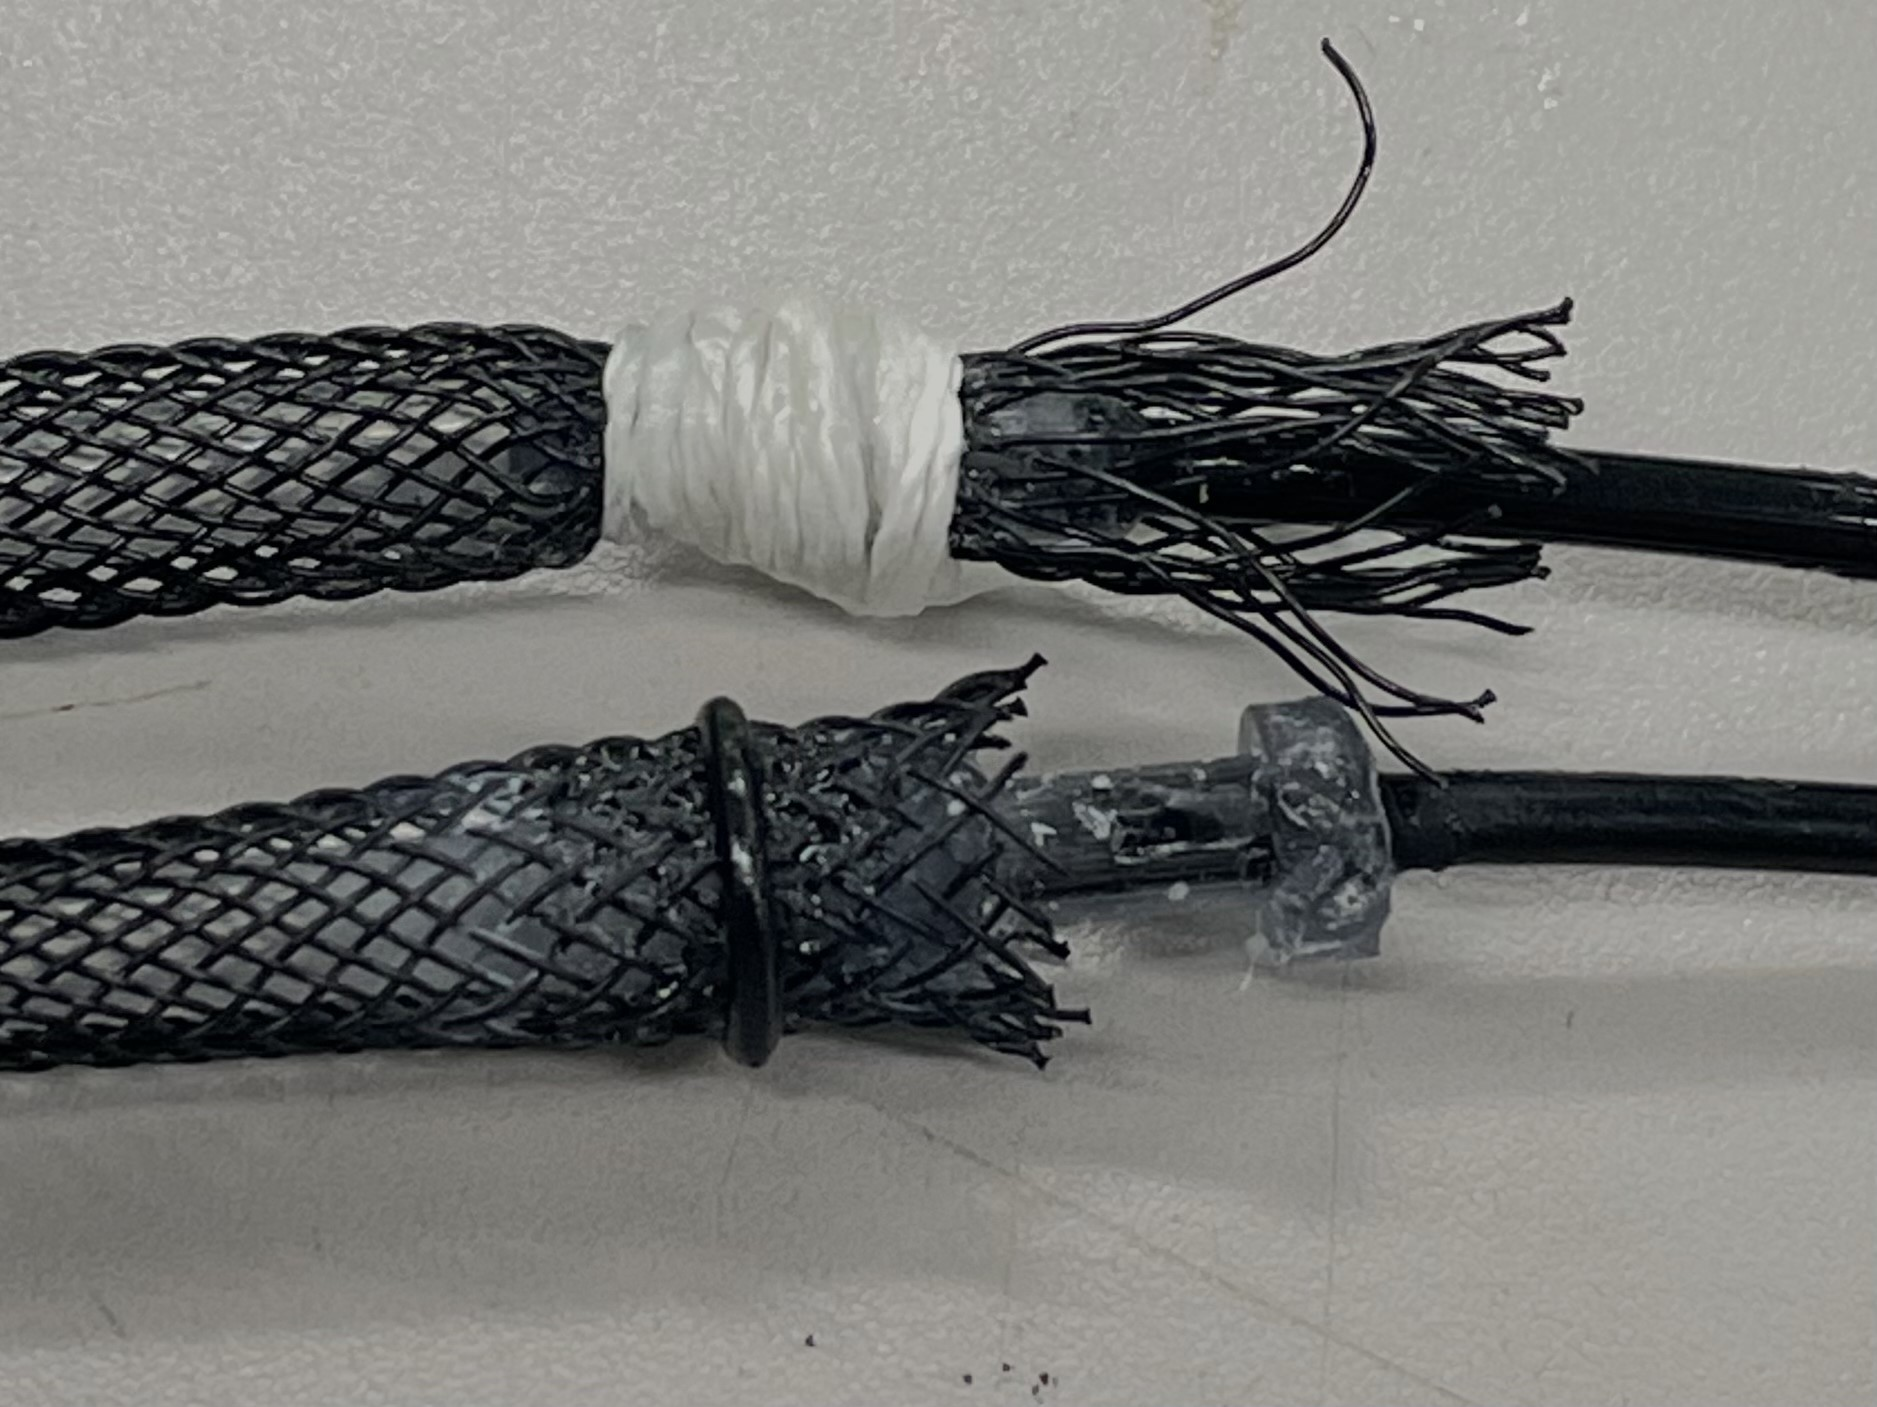
\includegraphics[scale=0.05]{mpa_oring_1.jpg}
    \vspace{-8mm}
    \caption{細径MPA}
    \label{fig:OringMPA}
  \end{minipage}
  \hspace{0.04\columnwidth}
  \begin{minipage}[b]{0.47\columnwidth}
    \centering
    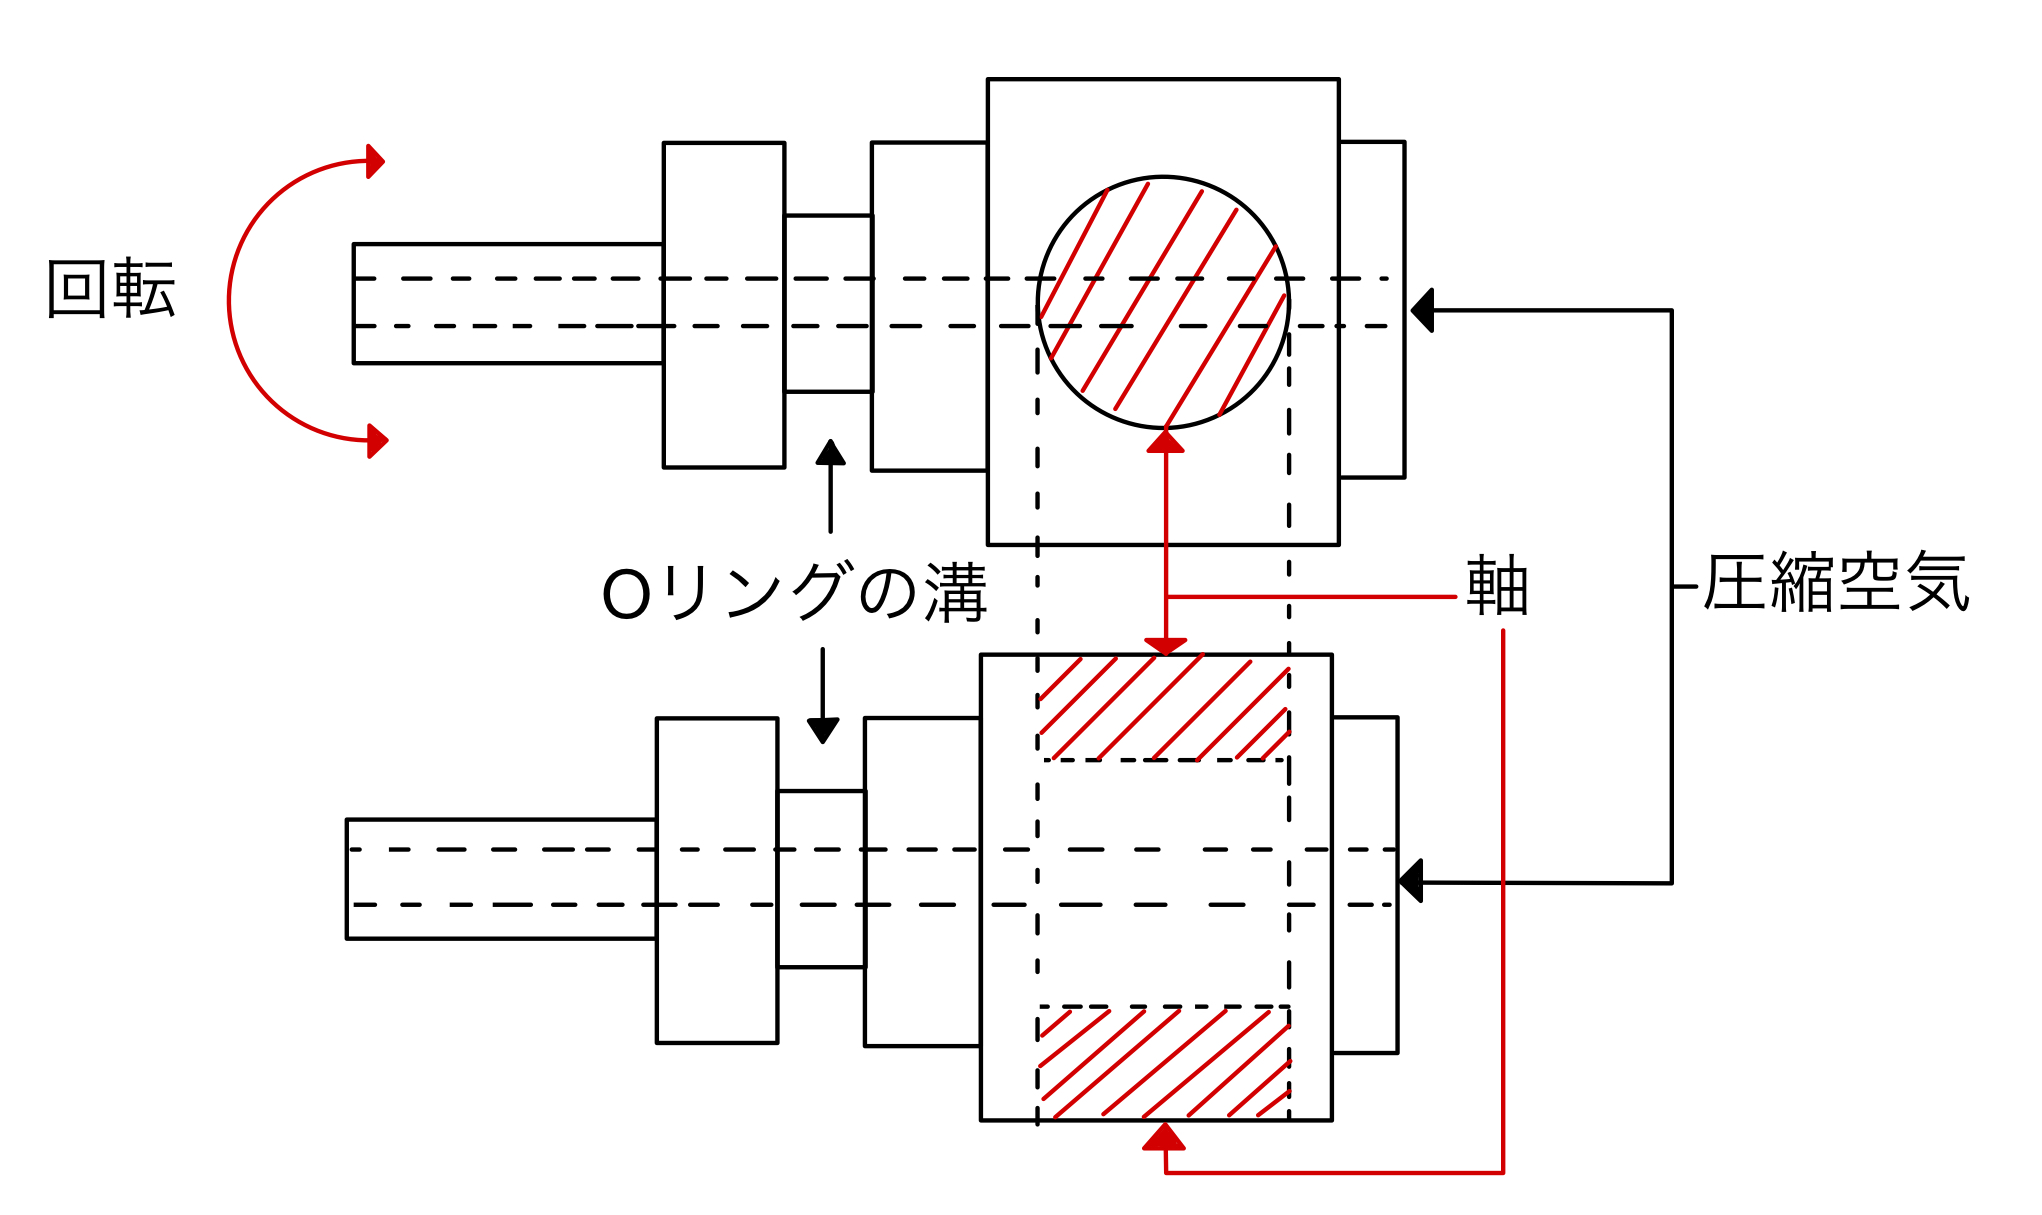
\includegraphics[scale=0.05]{MPA_irast.jpg}
    \vspace{-5mm}
    \caption{細径MPA端部部品}
    \label{fig:MPAparts}
  \end{minipage}
\end{figure}
%%%%%%%%%%%%%%%%%%%%%%%%%%%%%%%%%%%%%%%%%%%%%%%%%%%%%%%%%%%%%%%%%%%%%%%%%%%%%%%

現することができなかったので,以下のような改良を行った.
%%%%%%%%%%%%%%%%%%%%%%%%%%%%%%%%%%%%%%%%%%%%%%%%%%%%%%%%%%%%%%%%%%%%%%%%%%%%%%%
\vspace*{-2mm}
\section{細径MPA作成方法}

\vspace*{-1mm}
\subsection{細径MPAの締結方法}

図\ref{fig:crabrobot}のロボットではでは図\ref{fig:OringMPA}の上のようにMPAの端部をPEラインと呼ばれる釣り糸を巻き付けその部分に接着剤を塗布することで細径MPAを作成していた.
この締結方法では時間がかかり,空気が漏れることがあった.そこで,図\ref{fig:OringMPA}の下のようにMPAの端部にOリングを付けその部分に
接着剤を塗布してMPAを試作してみたところ,製作時間を大幅に短縮でき空気が漏れることなく動作することを確認することができた.
これによりMPA作成時の効率が大幅に上がった.

%%%%%%%%%%%%%%%%%%%%%%%%%%%%%%%%%%%%%%%%%%%%%%%%%%%%%%%%%%%%%%%%%%%%%%%%%%%%%%%
\vspace*{-1mm}
\subsection{細径MPAの固定部品}

生物の筋肉は弛緩する際に筋肉の角度を変化させている.それを再現するために図\ref{fig:MPAparts}のような
細径MPAの端部の部品を作成した.この部品の赤い斜線部にある穴を回転の軸にして細径MPAの角度が自由に変化するという仕組みになっている.
これにより細径MPAが動作する時にMPAが端部の部品に干渉しないことが確認できた.

%%%%%%%%%%%%%%%%%%%%%%%%%%%%%%%%%%%%%%%%%%%%%%%%%%%%%%%%%%%%%%%%%%%%%%%%%%%%%%%
\vspace*{-1mm}
\subsection{伸び切った状態の細径MPAの作成}

細径MPAを市販のナイロンメッシュをそのまま用いて作成すると,完成した細径MPAのシリコンゴムチューブとナイロンメッシュの間に隙間が空いてしまう問題があった.
それを解決するために直径2mmのステンレス丸棒をナイロンメッシュの中に差し込んでホットプレートで温めた.これによりナイロンメッシュの直径を2mmにして隙間をなくすことができ,
収縮率を増加することができた.

%%%%%%%%%%%%%%%%%%%%%%%%%%%%%%%%%%%%%%%%%%%%%%%%%%%%%%%%%%%%%%%%%%%%%%%%%%%%%%%
\vspace*{-2mm}
\section{結言}

本稿では,外骨格生物模倣ロボットの開発をするにあたって課題となる細径MPA の作成方法と固定方法に対していくつかの部品を作製し改良を行った.
しかし,蟹の筋配置についての再現はできなかった.今後は,蟹の腱と筋肉の配置の分析を解剖の結果から行い,
それを再現することができる実機の作成を目指す.





%%%%%%%%%%%%%%%%%%%%%%%%%%%%%%%%%%%%%%%%%%%%%%%%%%%%%%%%%%%%%%%%%%%%%%%%%%%%%%%
%\begin{figure}[t]
%  \begin{minipage}[b]{0.47\columnwidth}
%    \centering
%    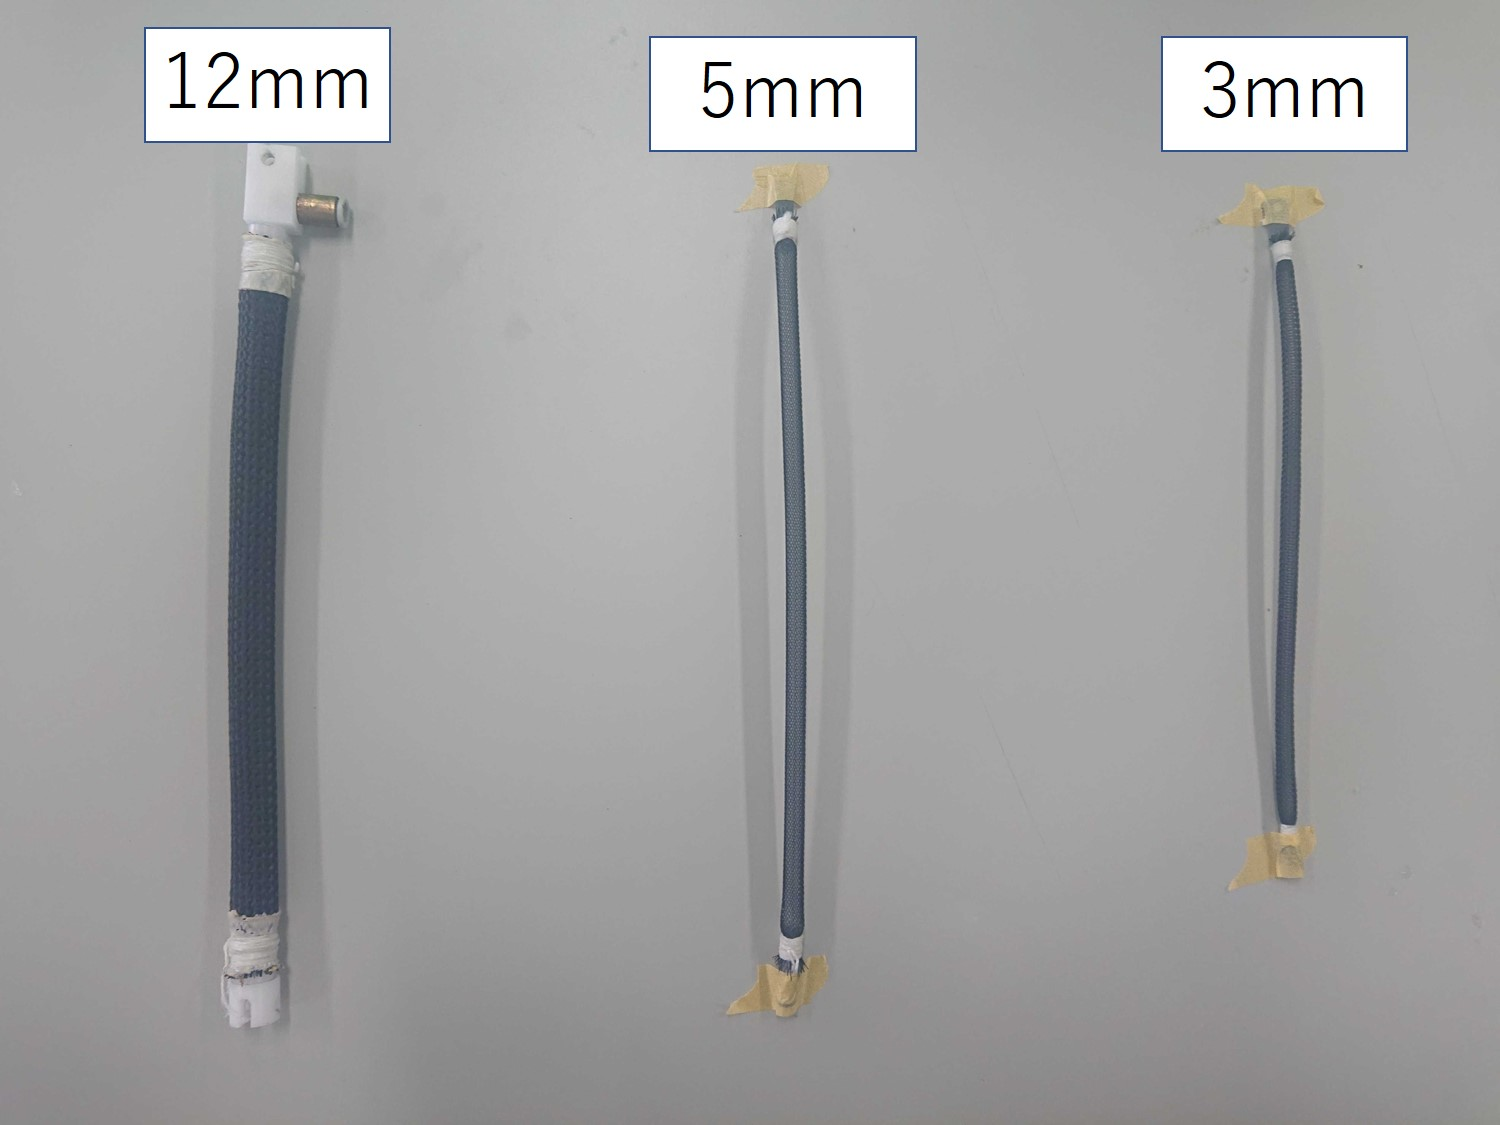
\includegraphics[scale=0.13]{mpa.JPG}
%    \vspace{-4mm}
%    \caption{MPAの外径}
%    \label{fig:MPA}
%  \end{minipage}
%  \hspace{0.04\columnwidth}
%  \begin{minipage}[b]{0.47\columnwidth}
%    \centering
%    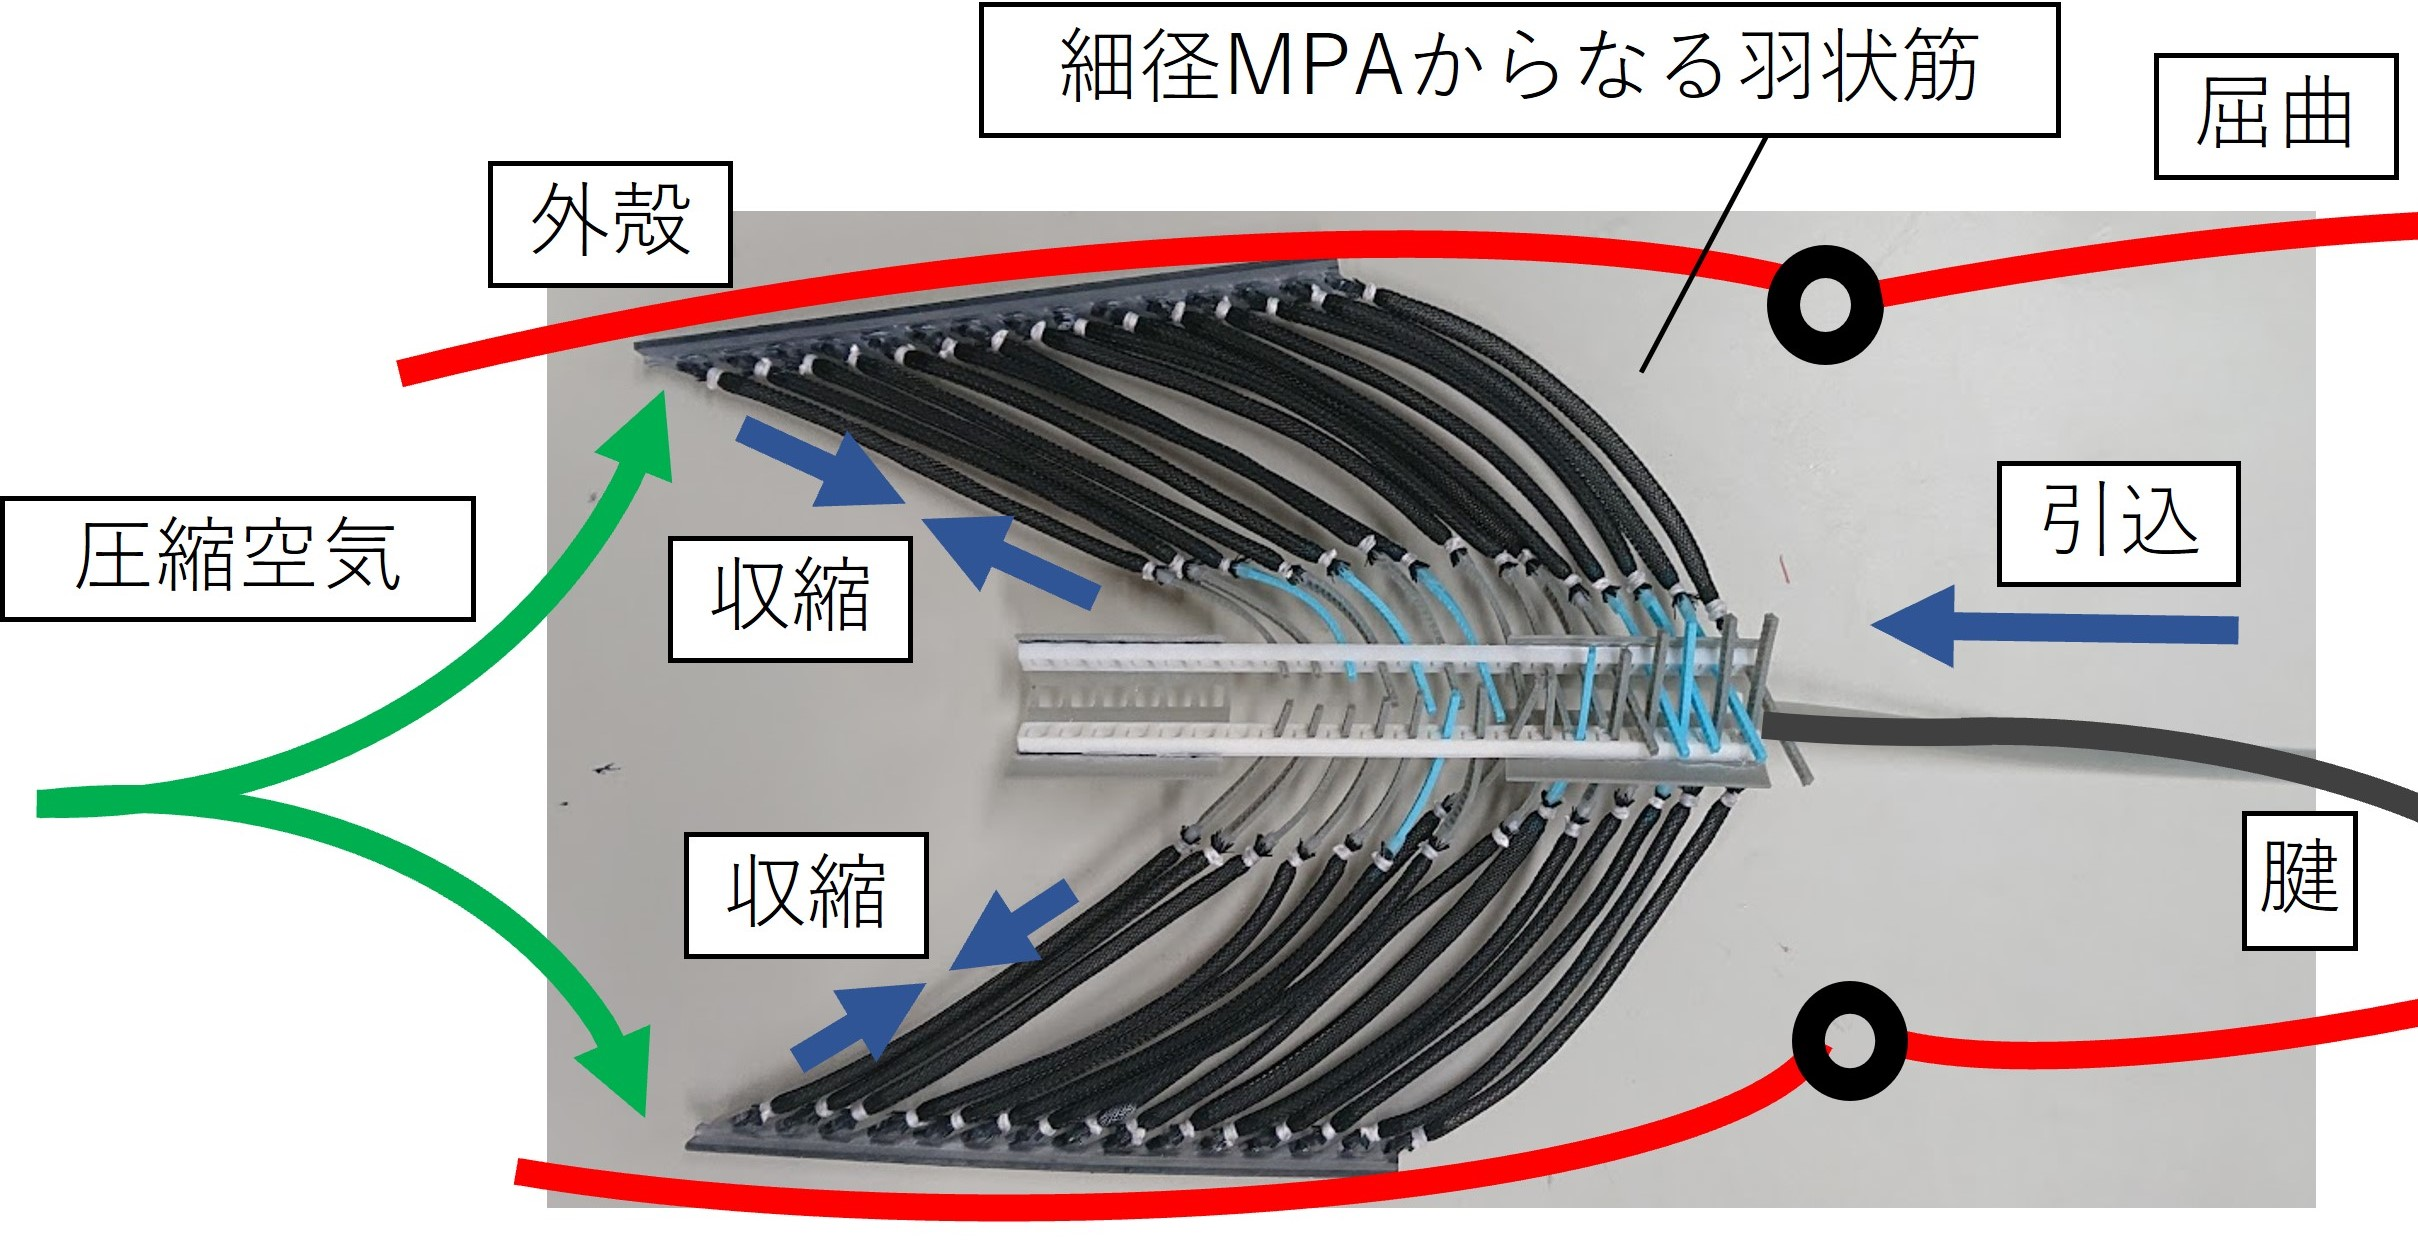
\includegraphics[scale=0.18]{mosiki.JPG}
%    \vspace{-2mm}
%    \caption{蟹模倣ロボット\cite{crabrobot2}}
%    \label{fig:crabrobot}
%  \end{minipage}
%\end{figure}
%%%%%%%%%%%%%%%%%%%%%%%%%%%%%%%%%%%%%%%%%%%%%%%%%%%%%%%%%%%%%%%%%%%%%%%%%%%%%%%

%%%%%%%%%%%%%%%%%%%%%%%%%%%%%%%%%%%%%%%%%%%%%%%%%%%%%%%%%%%%%%%%%%%%%%%%%%%%%%%
%\begin{figure}[t]
%  \begin{minipage}[b]{0.47\columnwidth}
%    \centering
%    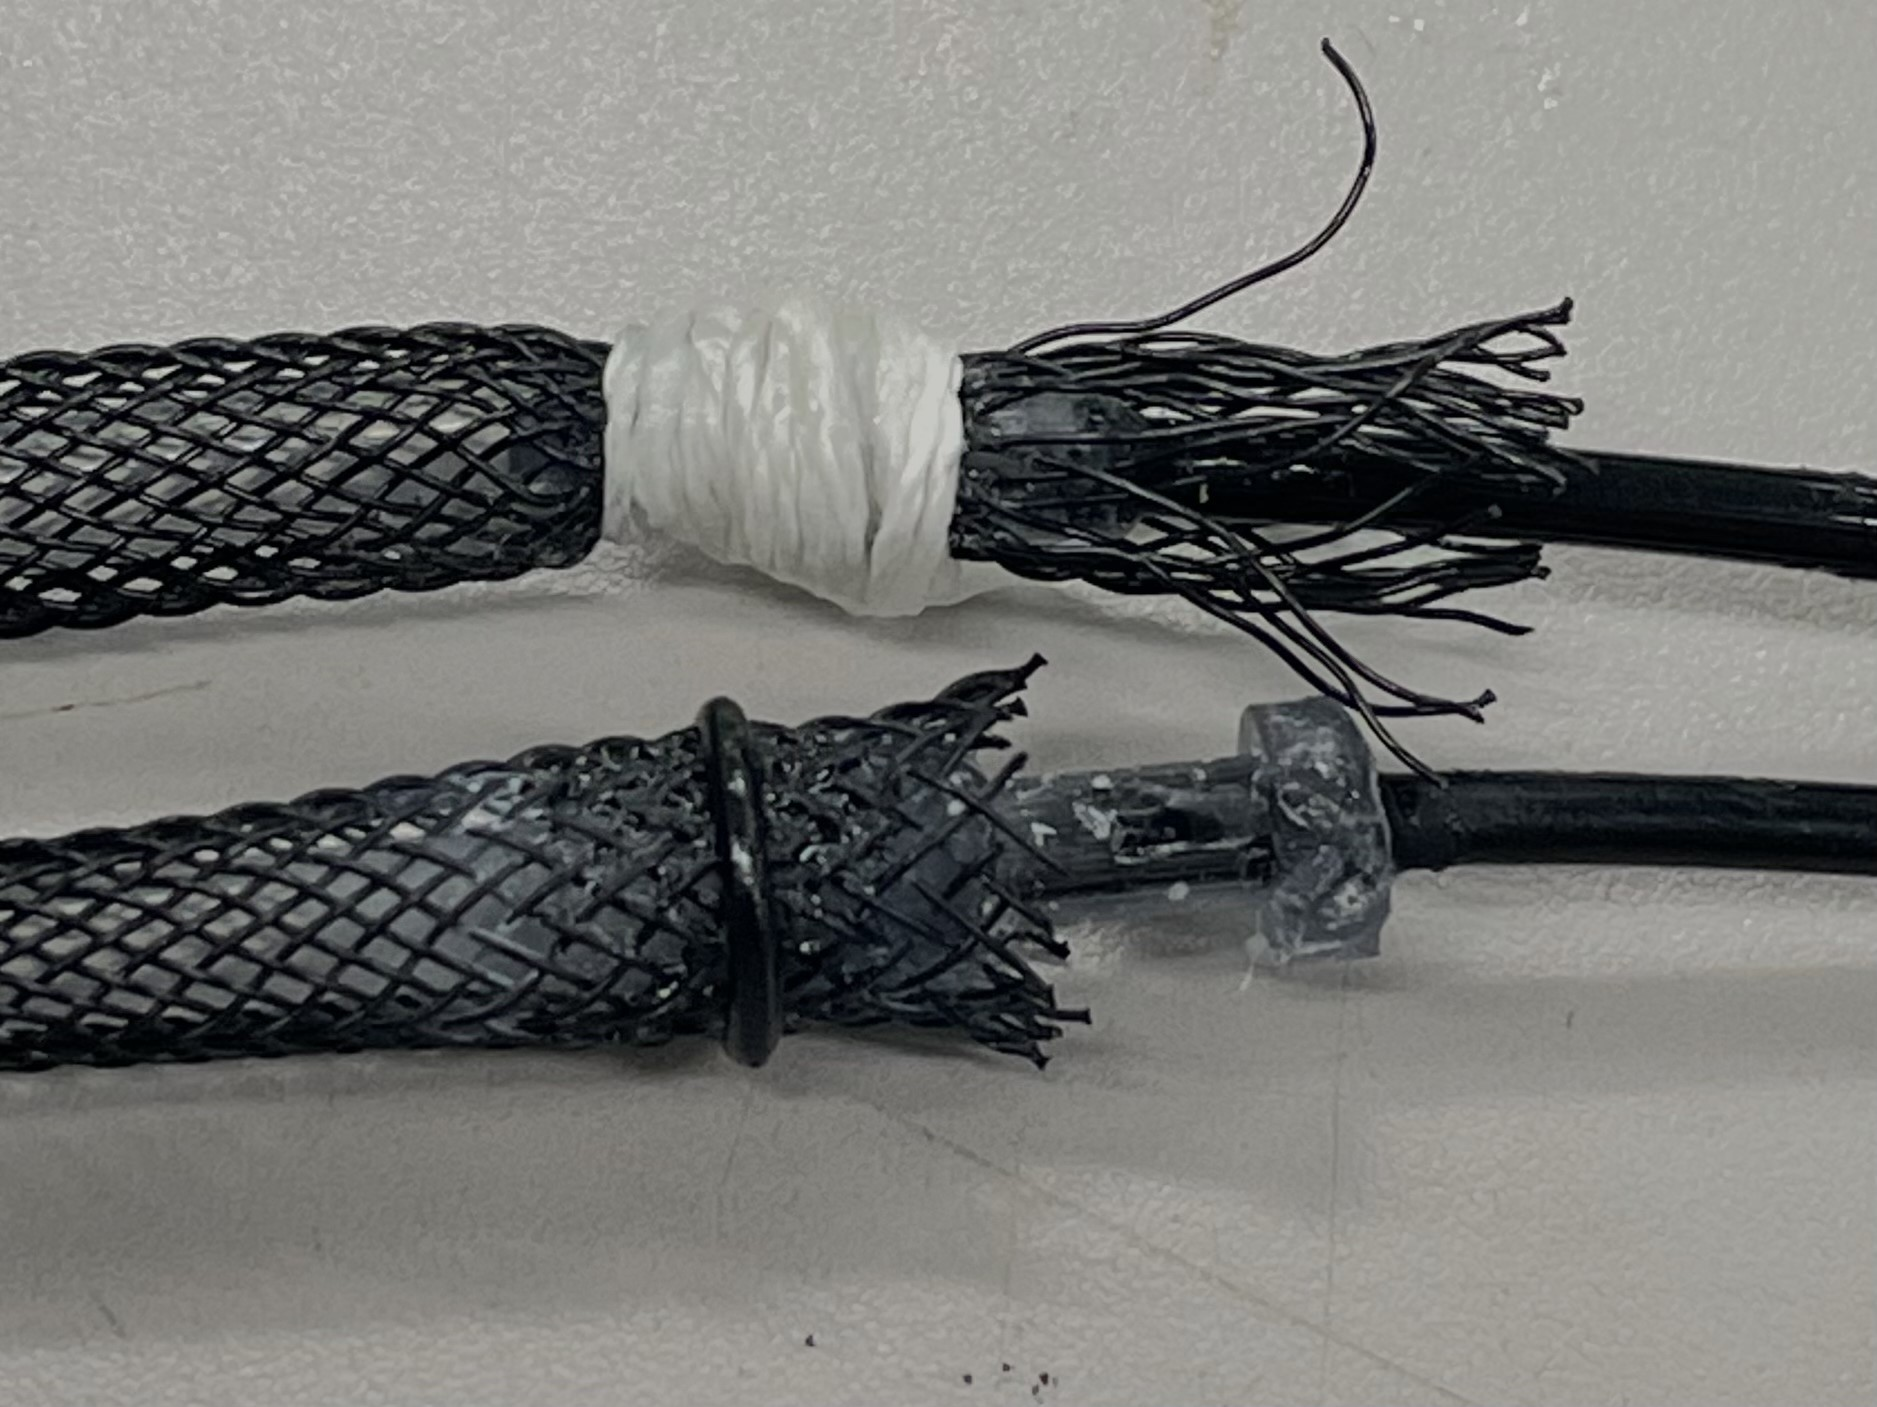
\includegraphics[scale=0.2]{mpa_oring_1.jpg}
%    \vspace{-8mm}
%    \caption{細径MPA}
%    \label{fig:OringMPA}
%  \end{minipage}
%  \hspace{0.04\columnwidth}
%  \begin{minipage}[b]{0.47\columnwidth}
%    \centering
%    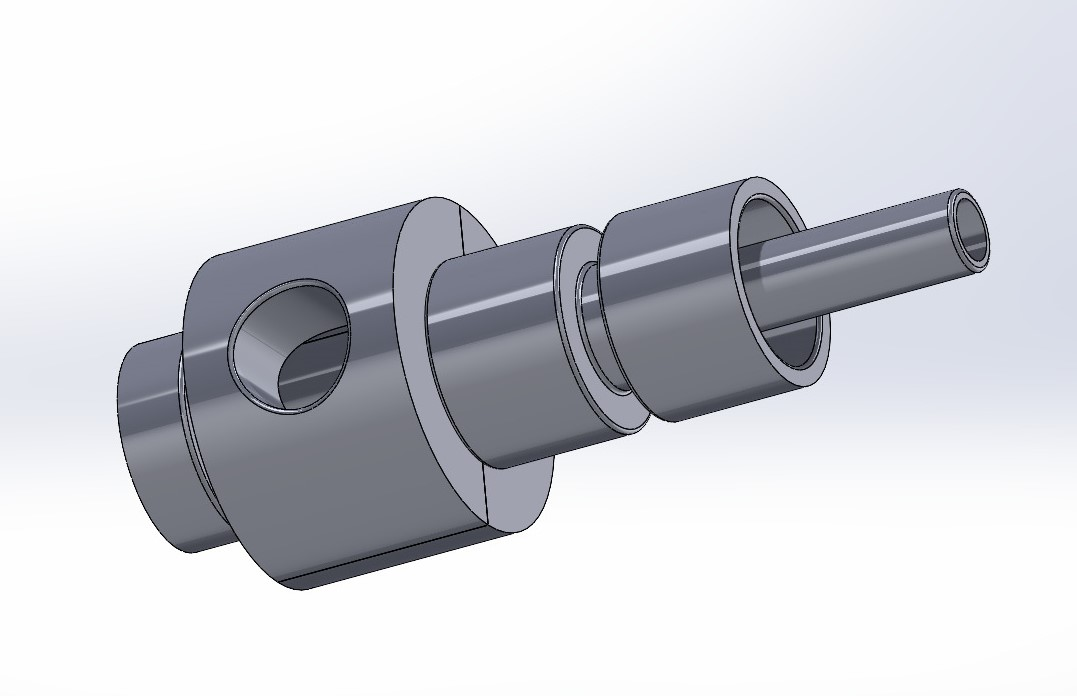
\includegraphics[scale=0.13]{MPAparts.JPG}
%    \vspace{-5mm}
%    \caption{細径MPA端部部品}
%    \label{fig:MPAparts}
%  \end{minipage}
%\end{figure}
%%%%%%%%%%%%%%%%%%%%%%%%%%%%%%%%%%%%%%%%%%%%%%%%%%%%%%%%%%%%%%%%%%%%%%%%%%%%%%%

%%%%%%%%%%%%%%%%%%%%%%%%%%%%%%%%%%%%%%%%%%%%%%%%%%%%%%%%%%%%%%%%%%%%%%%%%%%%%%%
\begin{thebibliography}{99}

  \bibitem{wakimoto}
  脇本修一,
  細径McKibben型人工筋の開発と用途開拓,
  計測と制御,57巻,11号,pp.812-815,2018
  
  \bibitem{crabrobot1}
  CHEN, Xi, et al. Study on the Design and Experimental Research on a Bionic Crab Robot with Amphibious Multi-Modal Movement, Journal of Marine Science and Engineering,10,12,p.1804,2022
  
  \bibitem{crabrobot2}
  中西大輔,長谷川侑大,浪花啓右,杉本靖博,
  細径空圧筋を用いた羽状筋および外骨格生物模倣ロボットの開発,ロボティクス・メカトロニクス講演会2024,2A1-L08,2024.

  % \bibitem{crab}
  % 佐藤武弘,自然科学のとびら,第17巻,1号,pp.7-8,2011
  
  
 \end{thebibliography}
 %%%%%%%%%%%%%%%%%%%%%%%%%%%%%%%%%%%%%%%%%%%%%%%%%%%%%%%%%%%%%%%%%%%%%%%%%%%%%%%
\end{document}